\ifdefined\standalone
\documentclass[12pt]{article}
\usepackage{graphicx}
\usepackage{float}
\usepackage[a4paper, margin=1in]{geometry}
\usepackage[utf8]{inputenc}
\usepackage{textcomp}
\usepackage{amsmath}
\usepackage{booktabs}
\usepackage{tikz}
\usepackage{enumitem}
\usetikzlibrary{decorations.pathmorphing,patterns}
\usepackage[hidelinks]{hyperref}
\usepackage[toc,page]{appendix}

\begin{document}
\fi


\section{Pure gas species diffusion}

This verification case evaluates the gas species transport solver in the limit of \emph{pure diffusion}. Numerical results are compared with an analytical solution for transient diffusion in a one-dimensional porous medium.

A one-dimensional porous layer of thickness $L = 1~\mathrm{m}$ is considered, with a uniform porosity $\overline{\psi}=0.6$. The temperature and pressure are spatially uniform and remain constant at $T=300~\mathrm{K}$ and $P=1~\mathrm{bar}$. Gas transport occurs solely by diffusion, with no advection and no volumetric source terms. The gaseous mixture consists of oxygen (O$_2$) and nitrogen (N$_2$), whose mass fractions are computed using the gas species diffusion solver. The external mass fractions are fixed to $Y_{\mathrm{O_2}}^{\infty}=0.22$ and $Y_{\mathrm{N_2}}^{\infty}=0.78$. Initially, the porous medium contains only nitrogen, such that $Y_{0,\mathrm{O_2}}=0$ and $Y_{0,\mathrm{N_2}}=1$ throughout the domain. Figure~\ref{fig:gas_species_diffusion} illustrates the configuration.


\begin{figure}[H]
\centering
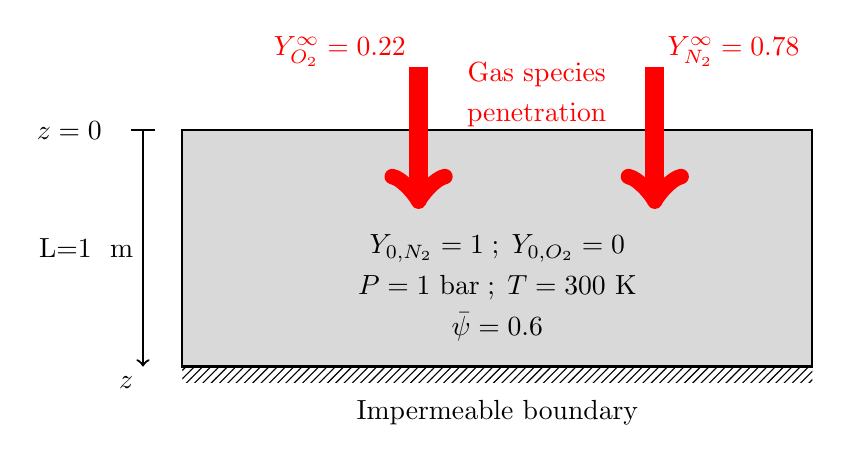
\begin{tikzpicture}[scale=1]

\draw[fill=gray!30,thick] (0,0) rectangle (8,3); 

\node at (4,1) {$P = 1~\mathrm{bar}  \; ; \;  T = 300~\mathrm{K}$};
\node at (4,0.5) {$\bar{\psi} = 0.6$};
\node at (4,1.5) {$Y_{0,N_2} = 1 \; ; \; Y_{0,O_2} = 0$};


\draw[thick] (-0.35,3) -- (-0.65,3); 
\node[left] at (-0.9,3) {$z=0$};

\draw[thick,->] (-0.5,3) -- (-0.5,0);
\node[left] at (-0.5,1.5) {L=1~ m};
\node[left] at (-0.5,-0.2) {$z$};



\node[red] at (7,4) {$Y_{N_2}^{\infty} = 0.78$};
\node[red] at (2,4) {$Y_{O_2}^{\infty} = 0.22$};

\draw[red,line width=7pt,->] (3,3.8) -- (3,2);
\draw[red,line width=7pt,->] (6,3.8) -- (6,2);
\node[red] at (4.5,3.7) {Gas species};
\node[red] at (4.5,3.2) {penetration};
\fill[pattern=north east lines] (0,-0.2) rectangle (8,0);
\node[below] at (4,-0.3) {Impermeable boundary};

\end{tikzpicture}
\caption{Configuration schematic}
\label{fig:gas_species_diffusion}
\end{figure}



Under these assumptions, the transport equation for each gaseous species reduces to the diffusion equation
\begin{equation}
\frac{\partial Y_j}{\partial t} = D\,\nabla^2 Y_j
\end{equation}
where $Y_j$ is the species mass fraction and $D$ is the effective diffusivity. Note that this equation is mathematically equivalent to the transient heat conduction equation.

The bottom boundary ($z=L$) is impermeable to diffusion:
\begin{equation}
\left. \partial_z Y_j \right|_{z=L} = 0.
\end{equation}

At the top boundary ($z=0$), a convective boundary condition is imposed:
\begin{equation}
-\bigl[\overline{\psi}\,\rho_g\,D\,\partial_z Y_j\bigr]_{z=0} = h_m\,\bigl(Y_j^{\infty} - Y_j(0,t)\bigr)
\end{equation}
where the mass transfer coefficient $h_m$ is expressed in $\mathrm{kg\, m^{-2}\, s^{-1}}$.

Assuming a semi-infinite medium, the analytical solution of this problem is given by \cite{incropera_fundamentals_2007}:
\begin{equation}
Y_j(z,t) = Y_{0,j} - \bigl(Y_{0,j} - Y_j^{\infty}\bigr)\,\Phi(z,t)
\end{equation}
where the dimensionless function $\Phi(z,t)$ is defined as:
\begin{equation}
\Phi(z,t) = \operatorname{erfc}\!\left(\frac{z}{2\sqrt{D~t}}\right)
- \exp\!\left(\alpha z + \alpha^2 D t\right)
\operatorname{erfc}\!\left(\frac{z}{2\sqrt{D~t}} + \alpha\sqrt{D~t}\right)
\end{equation}
and $\alpha = \frac{h_m}{\overline{\psi}\,\rho_g\,D}$. 



The effective gas diffusivity is evaluated using the Chapman--Enskog model. The required gas molecular properties are reported in Table~\ref{tab:properties_diffusivity_gas}. Under the present thermodynamic conditions, the diffusivity is uniform and equal to $D = 0.20~\mathrm{cm^2\, s^{-1}}$.

\begin{table}[H]
\centering
\caption{Gas molecular properties}
\label{tab:properties_diffusivity_gas}
\begin{tabular}{@{}lccc@{}}
\toprule
Species & $M$ ($\mathrm{g\,mol^{-1}}$) & $\sigma$ ($\mathrm{\AA}$) & $\epsilon/k$ ($\mathrm{K}$) \\
\midrule
O$_2$ & 32 & 3.433 & 113 \\
N$_2$ & 28 & 3.681 & 91.5 \\
\bottomrule
\end{tabular}
\end{table}


Two values of the mass transfer coefficient are investigated: $h_m=0.01~\mathrm{kg\, m^{-2}\, s^{-1}}$ and $h_m=10^{-4}~\mathrm{kg\, m^{-2}\, s^{-1}}$.

For $h_m = 0.01~\mathrm{kg\, m^{-2}\, s^{-1}}$, the surface resistance is negligible compared with diffusive transport inside the porous medium. In this regime, the boundary condition effectively reduces to a Dirichlet condition and the surface mass fractions rapidly converge towards the imposed external values $Y_j^{\infty}$. This case therefore corresponds to fixed external concentrations.

Figures~\ref{fig:diffusion_hm01} and~\ref{fig:diffusion_hm0001} present the evolution of the O$_2$ and N$_2$ mass fraction profiles for both values of $h_m$. Numerical results are compared with the analytical solution at several times, demonstrating excellent agreement.

\begin{figure}[H]
\centering
\begin{minipage}{0.49\textwidth}
  \includegraphics[width=\textwidth]{hm_01/O2_Diffusion_hm01.png}
\end{minipage}
\hfill
\begin{minipage}{0.49\textwidth}
  \includegraphics[width=\textwidth]{hm_01/N2_Diffusion_hm01.png}
\end{minipage}
\caption{Species diffusion with $h_m = 0.01~\mathrm{kg\, m^{-2}\, s^{-1}}$.}
\label{fig:diffusion_hm01}
\end{figure}

\begin{figure}[H]
\centering
\begin{minipage}{0.49\textwidth}
  \includegraphics[width=\textwidth]{hm_0001/O2_Diffusion_hm0001.png}
\end{minipage}
\hfill
\begin{minipage}{0.49\textwidth}
  \includegraphics[width=\textwidth]{hm_0001/N2_Diffusion_hm0001.png}
\end{minipage}
\caption{Species diffusion with $h_m = 10^{-4}~\mathrm{kg\, m^{-2}\, s^{-1}}$.}
\label{fig:diffusion_hm0001}
\end{figure}



\ifdefined\standalone
\end{document}
\fi

